\subjectPresentation{3}{XAI and Meteo}{color3}

\subjectDevelopment{Analyse truthfulness of Results}{
	\begin{itemize}
		\item Can we explain the ML models decisions on a human understandable way?
		\item If so, can we use XAI to identify relations between regions, how they influence each other?
	\end{itemize}
	\vfill
	\centering
	We used the Titan data from November 2023 and the UNetR++ convolutional neural network 
}{color3}

\subjectDevelopment{The Titan data}{
    21 channels of AROME images + 16 channels of ARPÈGE images
    \vfill
    \begin{figure}[h]
        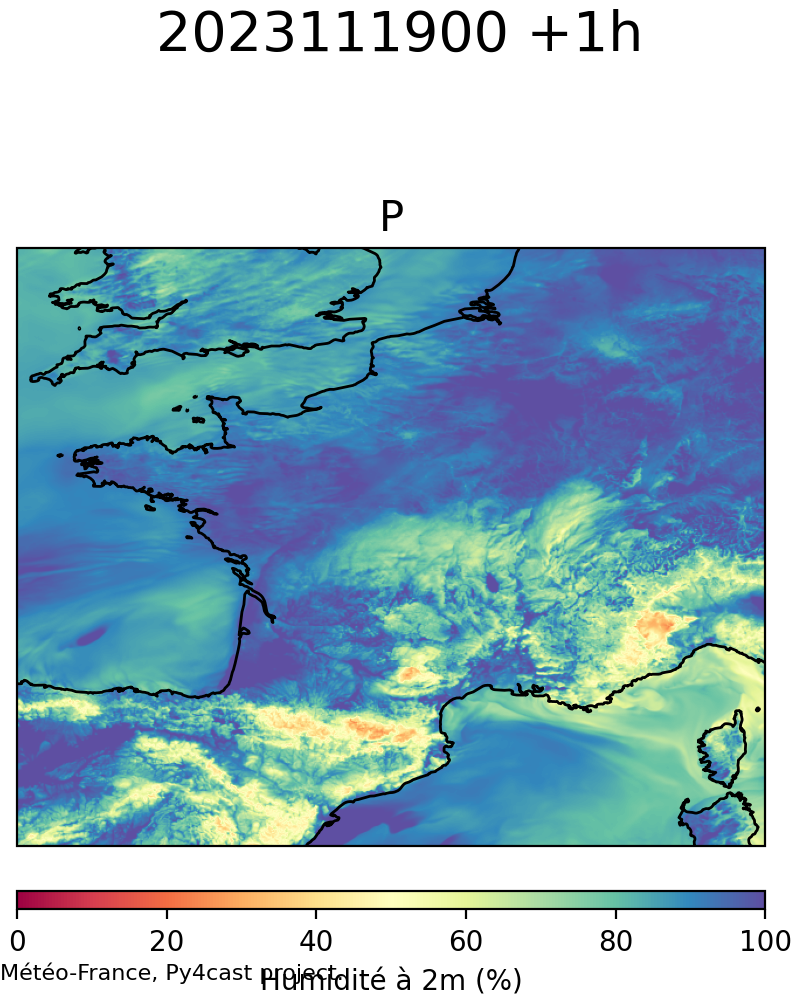
\includegraphics[width=0.2\textwidth]{Images/titan_data_examples/19_11/2023111900_feature_aro_r2_2m.png}
        \hfill
        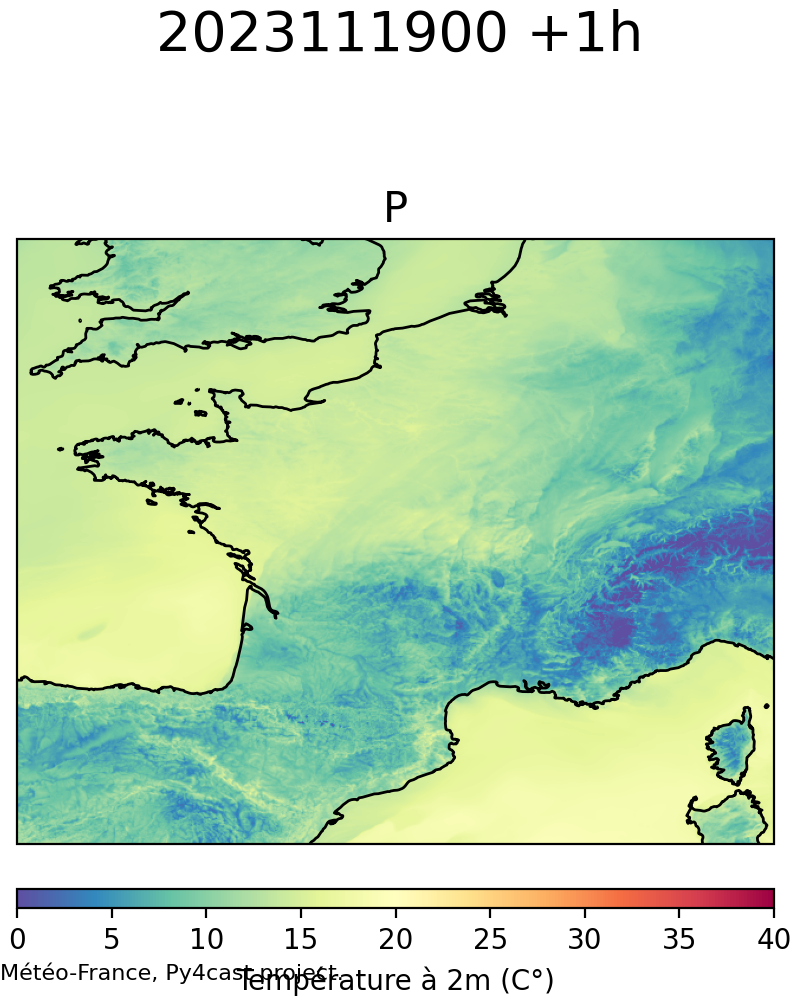
\includegraphics[width=0.2\textwidth]{Images/titan_data_examples/19_11/2023111900_feature_aro_t2m_2m.png}
        \hfill
        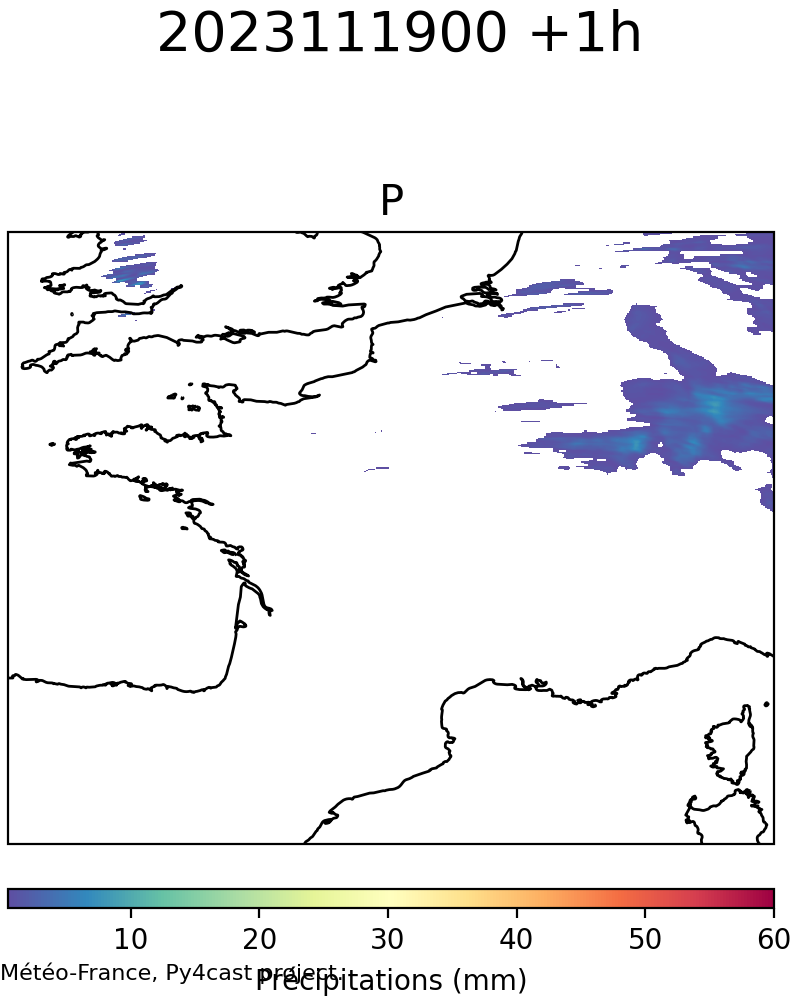
\includegraphics[width=0.2\textwidth]{Images/titan_data_examples/19_11/2023111900_feature_aro_tp_0m.png}
        \hfill
        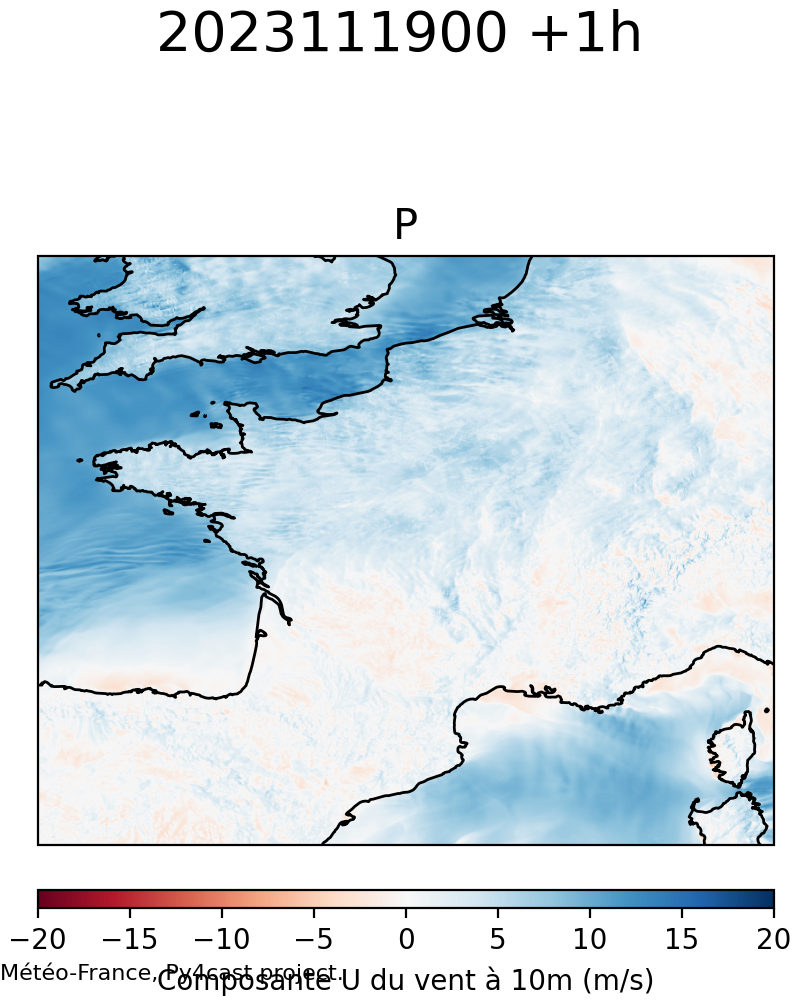
\includegraphics[width=0.2\textwidth]{Images/titan_data_examples/19_11/2023111900_feature_aro_u10_10m.png}
        \vfill
        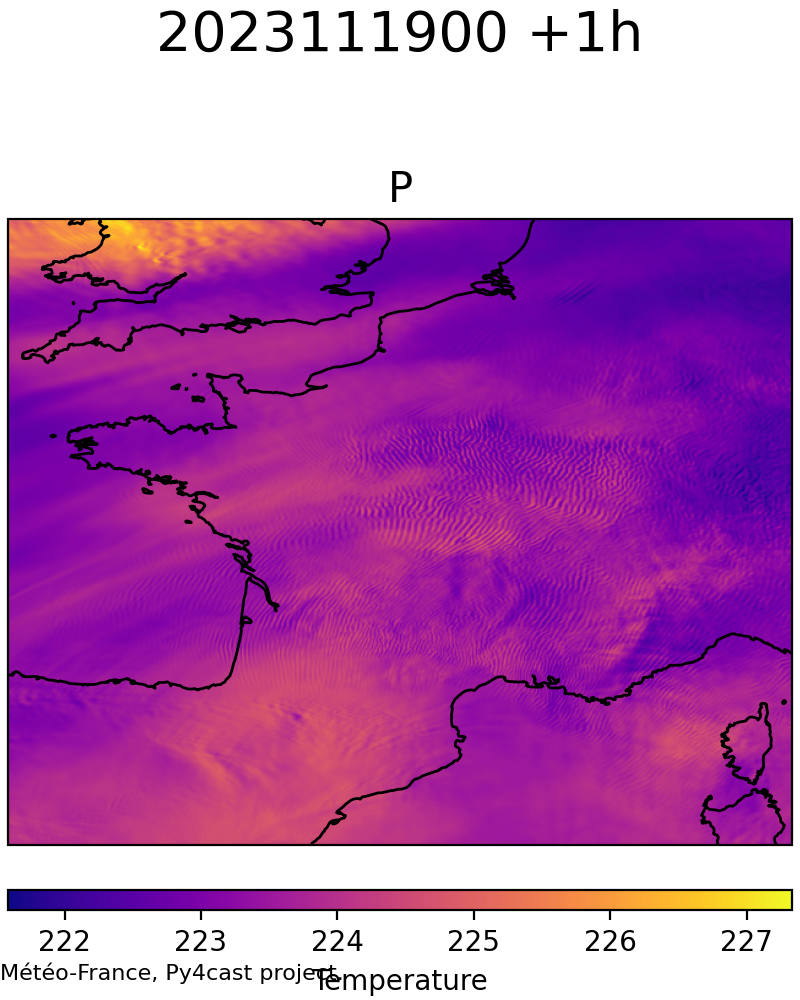
\includegraphics[width=0.2\textwidth]{Images/titan_data_examples/19_11/2023111900_feature_aro_t_250hpa.png}
        \hfill
        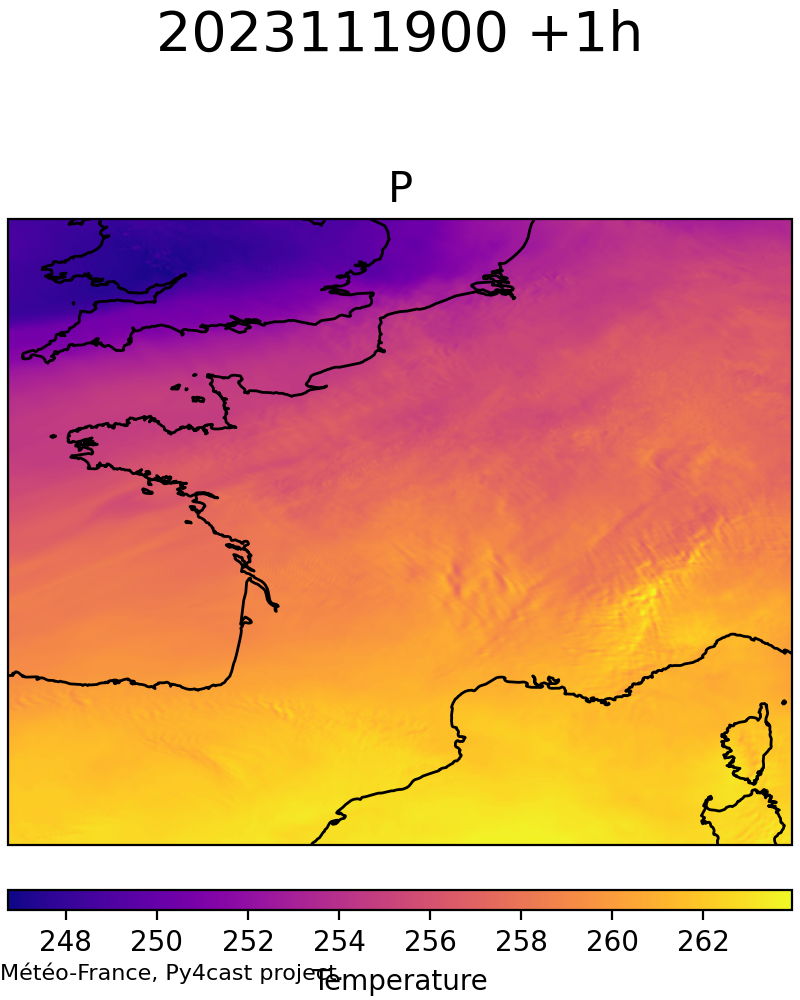
\includegraphics[width=0.2\textwidth]{Images/titan_data_examples/19_11/2023111900_feature_aro_t_500hpa.png}
        \hfill
        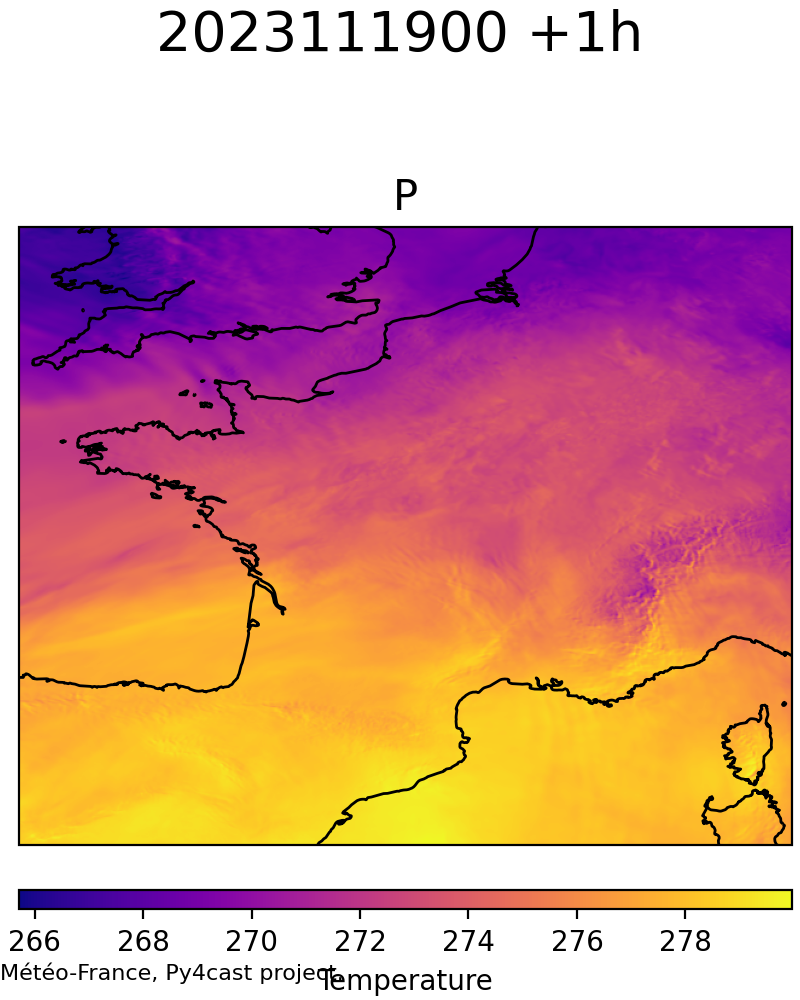
\includegraphics[width=0.2\textwidth]{Images/titan_data_examples/19_11/2023111900_feature_aro_t_700hpa.png}
        \hfill
        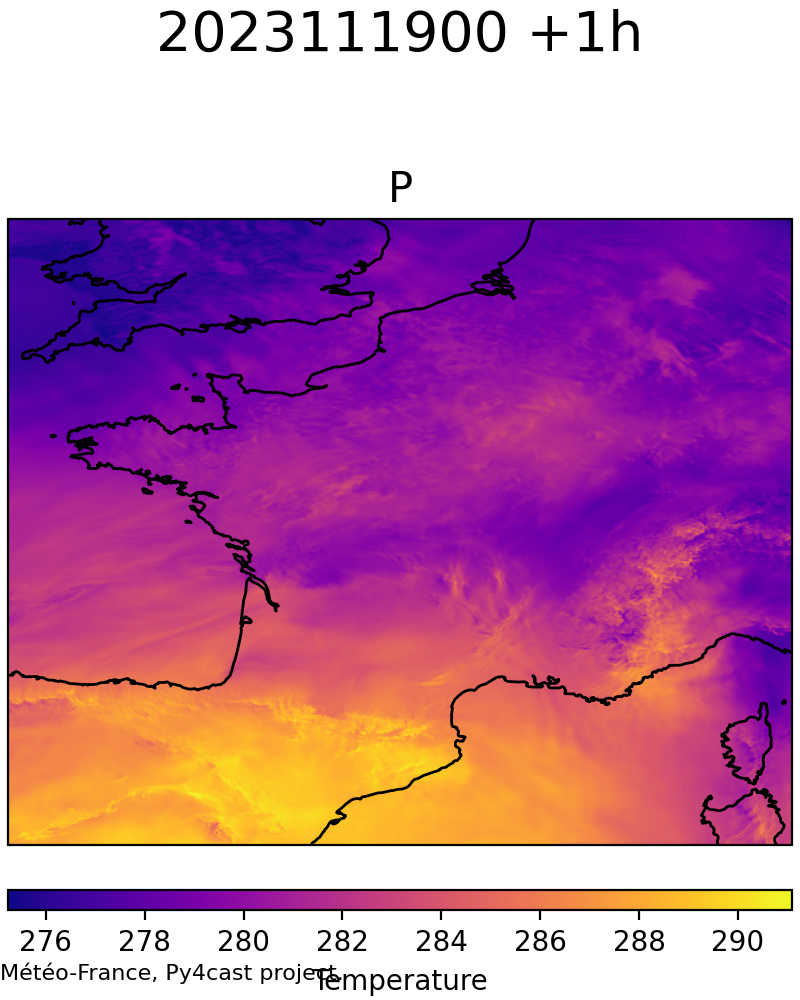
\includegraphics[width=0.2\textwidth]{Images/titan_data_examples/19_11/2023111900_feature_aro_t_850hpa.png}
        \caption{\scriptsize Titan image channels}
    \end{figure}
}{color3}

\subjectDevelopment{Combining AROME and ARPÈGE}{
Let $t$ be the present time and $t + 1$ be a future time.
\begin{itemize}
	\item Training without boundary conditions:
		\begin{itemize}
			\item Input: $aro_t$ (AROME at time $t$)
			\item Output: $aro_{t+1} - aro_t$ (The change in AROME from $t$ to $t+1$)
		\end{itemize}

	\item Training with boundary conditions:
		\begin{itemize}
			\item Input: $[aro_t, arp_t]$ (AROME and ARPÈGE at time $t$)
			\item Output: $aro_{t+1} - aro_t$ (The change in AROME from $t$ to $t+1$)
		\end{itemize}
\end{itemize}

In summary, the data can be combined in two primary ways: a simpler approach using only AROME data, and a more precise, operational-style approach that leverages \textbf{ARPÈGE data to provide essential boundary conditions}.
}{color3}

\subjectDevelopment{Py4cast Predictions}{
    \animategraphics[
        width=0.48\textwidth,
        autoplay,
        loop,
        palindrome
    ]{4}
    {Images/py4cast_predictions/frame_r2_}
    {001}
    {013}
    \hfill
    \animategraphics[
        width=0.48\textwidth,
        autoplay,
        loop,
        palindrome
    ]{4}
    {Images/py4cast_predictions/frame_tp_}
    {001}
    {013}
}{color3}

\subjectDevelopment{Applying Anchors on Weather Forecasting}{
We elaborated two extensions of the Anchors formalization, which will be particularly useful for the weather forecasting problem.

\begin{itemize}
	\item Deterministic Precision Constraint:

	\begin{equation}
		\arg \max_{A} {\text{cov}(A) \mid \text{prec}(A) \geq \tau }
		\label{eq:extended-max-cov-anchors}
	\end{equation}

	\item Extension to Regression and Probabilistic Output:
	
	\begin{equation}
		\text{prec}(A) = \mathbb{E}_{D(z|A)} [\mathbf{1}_{|f(x) - f(z)| > \tau}]
		\label{eq:extended-prec-anchors}
	\end{equation}

	where $\tau$ is a threshold above which the conditions of A are supposed to have a significant impact.
\end{itemize}
}{color3}

\subjectDevelopment{Generating data perturbations}{
    We suppose that $g_{i,j,c,R}(f(x_t)) == 1$, given a region $(i, j)$ in the map,  and we want to explain why using anchors. We will sample $K$ different counterfactual observations ${z_k}$, for $k \in {1, \ldots , K}$.

\begin{itemize}
	\item \textbf{Center of Perturbation:} $(\widehat{i_k}, \widehat{j_k})$
	
	\item \textbf{Channel of Perturbation:} $\widehat{c_k}$
	
	\item \textbf{Perturbation Value:} $\widehat{v_k}$
\end{itemize}
}{color3}

\subjectDevelopment{Perturbation Mask}{
    We introduce a second hyperparameter, $\sigma_e$, which models the spatial extent of the perturbation. The procedure for generating a counterfactual instance $z_k$ is then as follows:
\begin{itemize}
	\item \textbf{Unaffected Channels:} For all channels $c \neq \widehat{c_k}$, the data remains unchanged: $z_k(:, :, c) = x_t(:, :, c)$.
	
	\item \textbf{Mask Creation:} A mask $m \in \mathbb{R}^{I \times J}$ is generated. Its values are initially drawn from a 2D Gaussian distribution centered at $(\widehat{i_k}, \widehat{j_k})$ with covariance matrix $\begin{bmatrix} \sigma_e & 0 \ 0 & \sigma_e \end{bmatrix}$. These values are then linearly rescaled to the interval $[0, 1]$.
	
	\item \textbf{Application:} The perturbed channel $\widehat{c_k}$ in $z_k$ is created by a mask-based blending between the original values and the new value $\widehat{v_k}$:
	\begin{equation}
		z_k(\overline{i} , \overline{j} , \widehat{c_k}) = m(\overline{i} , \overline{j} ) * \widehat{v_k} + (1 - m(\overline{i} , \overline{j})) * x_t(\overline{i} , \overline{j}, \widehat{c_k})
		\label{eq:anchor-perturbation}
	\end{equation}
	for all $\overline{i} \in {1, \ldots, I}$ and $\overline{j} \in {1, \ldots, J}$.
\end{itemize}
}{color3}

\subjectDevelopment{Example of a Perturbed Image}{
\begin{figure}[h]
    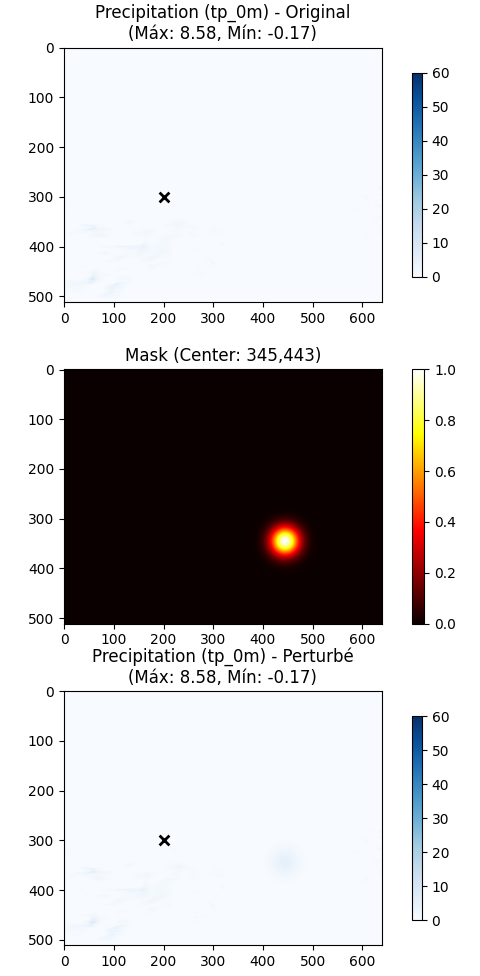
\includegraphics[width=0.3\textwidth]{Images/titan_rain_perturbations/perturbed_c_tp_0m.png}
    \hfill
    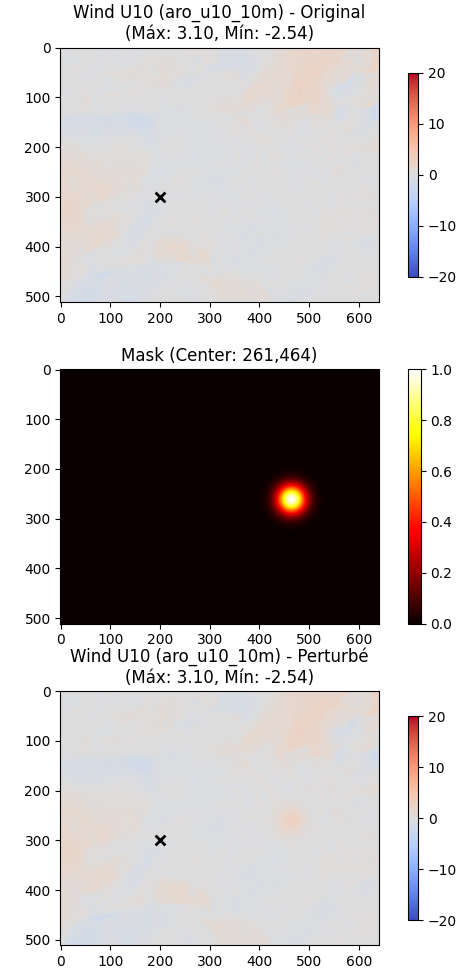
\includegraphics[width=0.3\textwidth]{Images/titan_rain_perturbations/perturbed_c_u10_10m.png}
    \hfill
    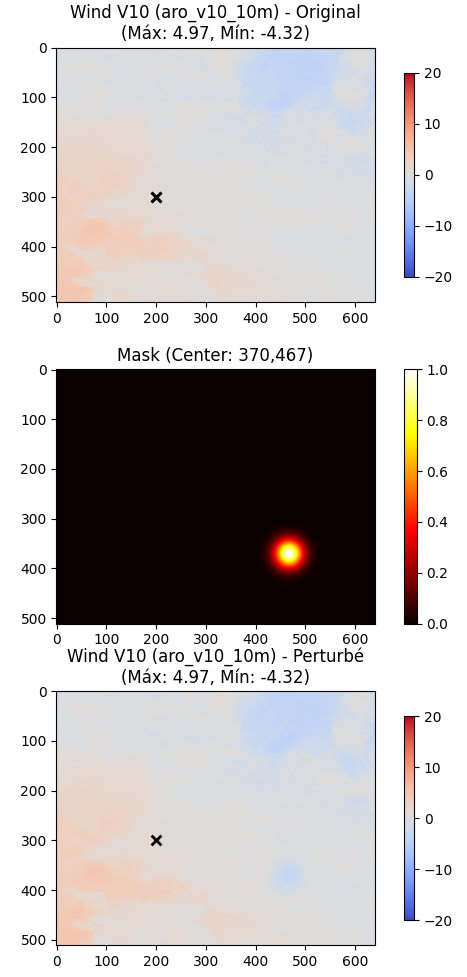
\includegraphics[width=0.3\textwidth]{Images/titan_rain_perturbations/perturbed_c_v10_10m.png}
    \caption{Example of counterfactuals of Titan image channels from 18/11/2023}
    \label{fig:titan-rain-perturbations}
\end{figure}
}{color3}

\subjectDevelopment{Running the Regression Anchors}{
    We generated about 300 conterfactuals per channel, in a radius of about \textbf{300 km from the target point}.
    \vfill
    Using a \textbf{mask of 40 km} for the perturbations.
    \vfill
    Seeing if the \textbf{rain prediction changed} in more than 5\%.
}{color3}

\subjectDevelopment{Rain Model}{
\begin{itemize}
    \item \textit{aro\_tp\_0m} (Total Precipitation)
	\item \textit{aro\_u10\_10m} (Zonal wind component at 10m)
    \item \textit{aro\_v10\_10m} (Meridional wind component at 10m)
\end{itemize}
}{color3}

\subjectDevelopment{Region of Chateaubriant on $18^{th}$ November}{
\begin{figure}[h]
    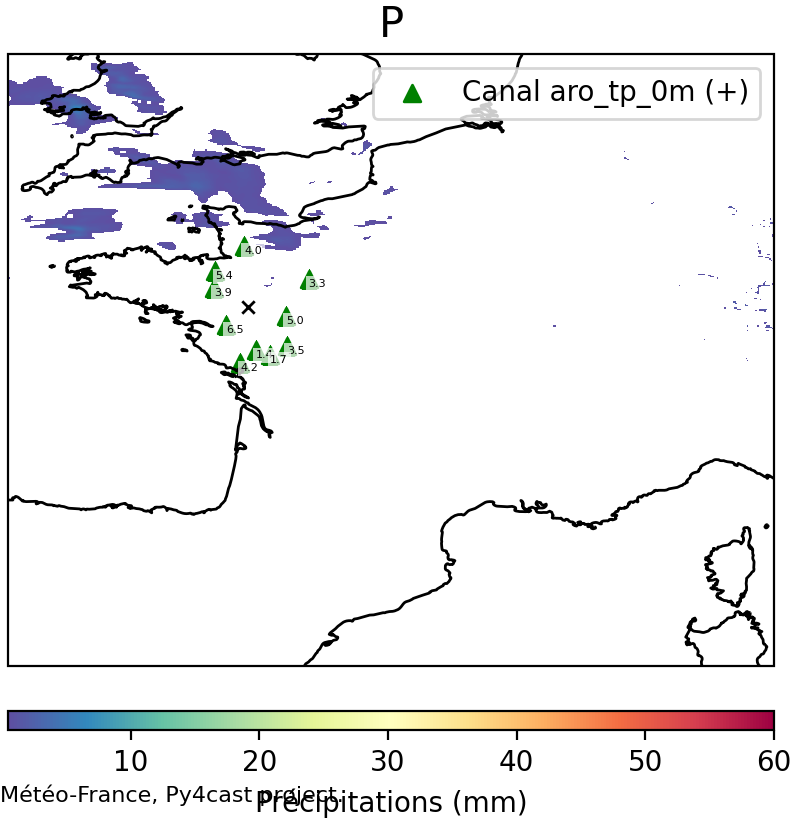
\includegraphics[width=0.38\textwidth]{Images/titan_rain_anchors/nov-18/2023111800_feature_aro_tp_0m.png}
    \hfill
    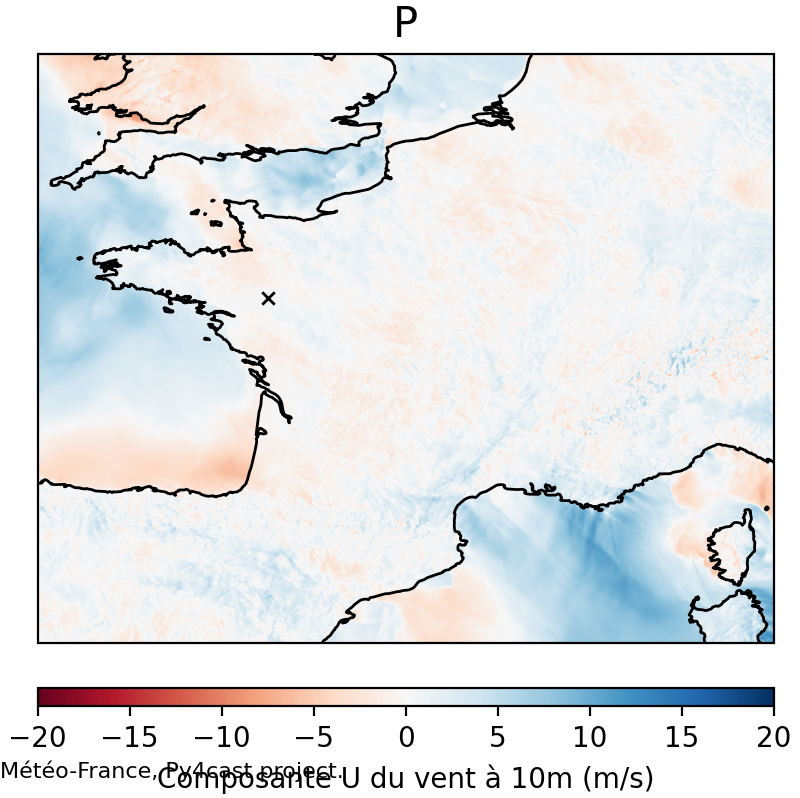
\includegraphics[width=0.38\textwidth]{Images/titan_rain_anchors/nov-18/2023111800_feature_aro_u10_10m.png}
    \hfill
    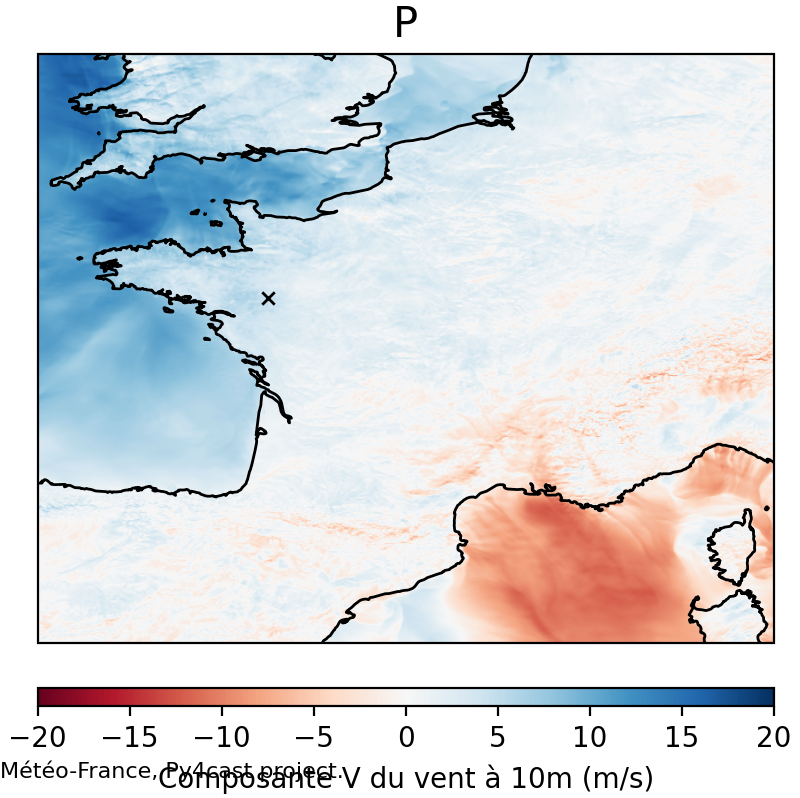
\includegraphics[width=0.38\textwidth]{Images/titan_rain_anchors/nov-18/2023111800_feature_aro_v10_10m.png}
\end{figure}
}{color3}

\subjectDevelopment{Region of Limoges on $21^{st}$ November}{
\begin{figure}[h]
    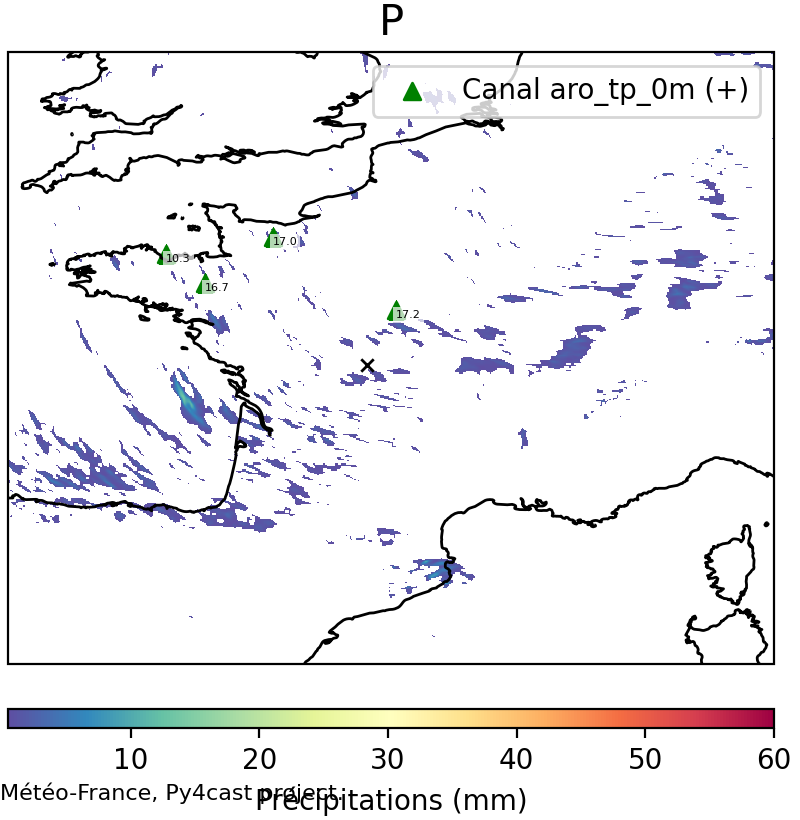
\includegraphics[width=0.38\textwidth]{Images/titan_rain_anchors/nov-21/2023112100_feature_aro_tp_0m.png}
    \hfill
    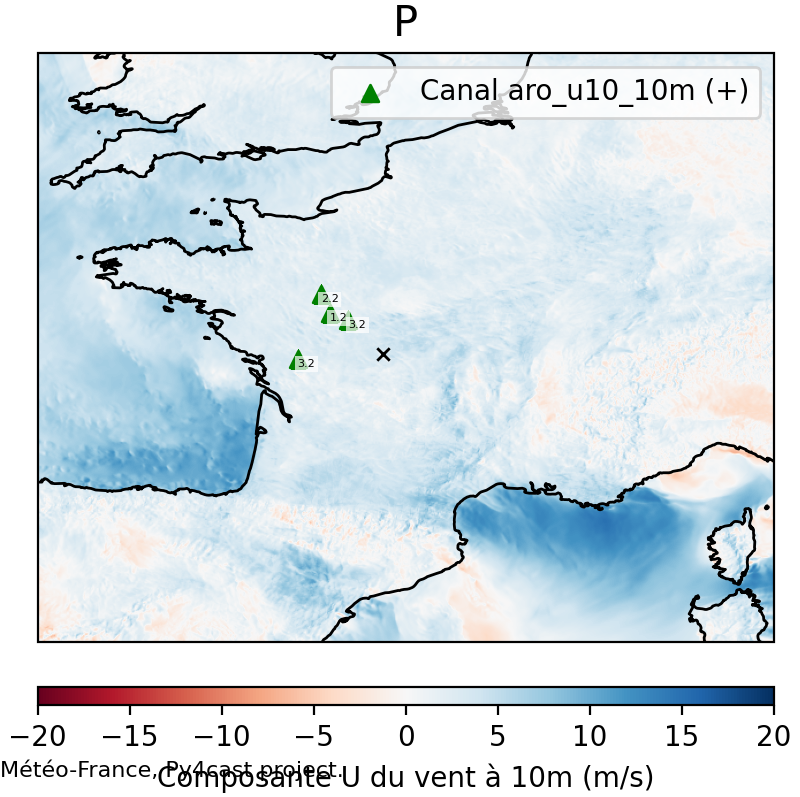
\includegraphics[width=0.38\textwidth]{Images/titan_rain_anchors/nov-21/2023112100_feature_aro_u10_10m.png}
    \hfill
    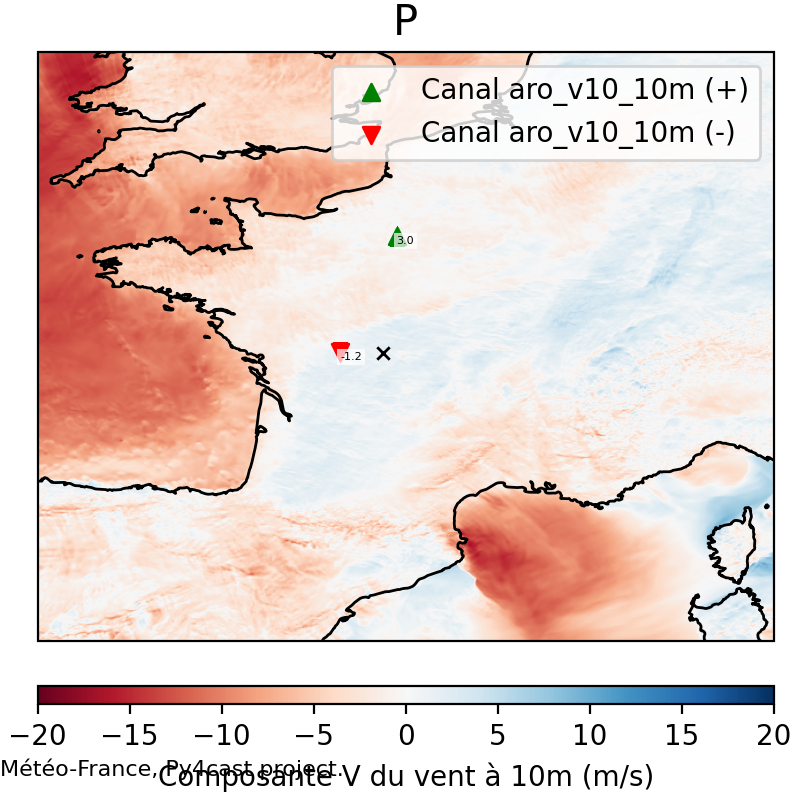
\includegraphics[width=0.38\textwidth]{Images/titan_rain_anchors/nov-21/2023112100_feature_aro_v10_10m.png}
    \caption{Example of anchors applied on "rain" channels, on $21^{st}$ November data.}
    \label{fig:titan-rain-anchors-21}
\end{figure}
}{color3}